\documentclass[12pt]{article}
\usepackage[margin=1in]{geometry}
\usepackage{subcaption}
\usepackage{graphicx}
\usepackage{placeins}
\usepackage{amsmath}
\usepackage{url}
\usepackage{cite}


% acronyms for text or math mode
% \newcommand {\ccast} {\mbox{\small\textsc{ccast}}}
\newcommand {\ccast} {\mbox{\small CCAST}}
\newcommand {\nedn} {\mbox{\small NEdN}}
\newcommand {\kcarta} {\mbox{k\small{CARTA}}}

\newcommand {\chirp} {\mbox{\small CHIRP}}
\newcommand {\cris}  {\mbox{\small CrIS}}
\newcommand {\airs}  {\mbox{\small AIRS}}
\newcommand {\iasi}  {\mbox{\small IASI}}
\newcommand {\idps}  {\mbox{\small IDPS}}
\newcommand {\nasa}  {\mbox{\small NASA}}
\newcommand {\noaa}  {\mbox{\small NOAA}}
\newcommand {\nstar} {\mbox{\small STAR}}
\newcommand {\umbc}  {\mbox{\small UMBC}}
\newcommand {\uw}    {\mbox{\small UW}}

\newcommand {\fft}  {\mbox{\small FFT}}
\newcommand {\ifft} {\mbox{\small IFFT}}
\newcommand {\fir}  {\mbox{\small FIR}}
\newcommand {\fov}  {\mbox{\small FOV}}
\newcommand {\for}  {\mbox{\small FOR}}
\newcommand {\ict}  {\mbox{\small ICT}}
\newcommand {\ils}  {\mbox{\small ILS}}
\newcommand {\igm}  {\mbox{\small IGM}}
\newcommand {\opd}  {\mbox{\small OPD}}
\newcommand {\rms}  {\mbox{\small RMS}}
\newcommand {\zpd}  {\mbox{\small ZPD}}
\newcommand {\ppm}  {\mbox{\small PPM}}
\newcommand {\srf}  {\mbox{\small SRF}}
\newcommand {\sdr}  {\mbox{\small SDR}}
\newcommand {\FWHM} {\mbox{\small FWHM}}
\newcommand {\fwhm} {\mbox{\small\textsc{fwhm}}}

\newcommand {\ES} {\mbox{\small ES}}
\newcommand {\SP} {\mbox{\small SP}}
\newcommand {\IT} {\mbox{\small IT}}
\newcommand {\SA} {\mbox{\small SA}}

\newcommand {\ET} {\mbox{\small ET}}
\newcommand {\FT} {\mbox{\small FT}}

\newcommand {\wn} {\mbox{cm$^{-1}$}}
\newcommand {\cm} {\mbox{cm}}

% abbreviations, mainly for math mode
\newcommand {\real} {\mbox{real}}
\newcommand {\imag} {\mbox{imag}}
\newcommand {\atan} {\mbox{atan}}
\newcommand {\obs}  {\mbox{obs}}
\newcommand {\calc} {\mbox{calc}}
\newcommand {\sinc} {\mbox{sinc}}
\newcommand {\psinc} {\mbox{psinc}}
\newcommand {\std} {\mbox{std}}
\newcommand {\nchan} {\mbox{nchan}}
\newcommand {\nobs} {\mbox{nobs}}

% symbols, for math mode only
\newcommand {\lmax} {L_{\mbox{\tiny max}}}
\newcommand {\vmax} {V_{\mbox{\tiny max}}}

\newcommand {\tauobs} {\tau_{\mbox{\tiny obs}}}
\newcommand {\taucal} {\tau_{\mbox{\tiny calc}}}
\newcommand {\Vdc}  {V_{\mbox{\tiny DC}}}

\newcommand {\rIT} {r_{\mbox{\tiny\textsc{ict}}}}
\newcommand {\rES} {r_{\mbox{\tiny\textsc{es}}}}
\newcommand {\robs} {r_{\mbox{\tiny obs}}}

\newcommand {\rITobs} {r_{\mbox{\tiny\textsc{ict}}}^{\mbox{\tiny obs}}}
\newcommand {\rITcal} {r_{\mbox{\tiny\textsc{ict}}}^{\mbox{\tiny cal}}}

\newcommand {\rESuser} {r_{\mbox{\tiny\textsc{es}}}^{\mbox{\tiny user}}}
\newcommand {\rITuser} {r_{\mbox{\tiny\textsc{ict}}}^{\mbox{\tiny user}}}
\newcommand {\rITsensor} {r_{\mbox{\tiny\textsc{ict}}}^{\mbox{\tiny sensor}}}
\newcommand {\rITfov} {r_{\mbox{\tiny\textsc{ict}}}^{\mbox{\tiny fov}}}

\newcommand {\fcos} {f_{\mbox{\tiny cos}}}
\newcommand {\fatbd} {f_{\mbox{\tiny\textsc{atbd}}}}

\newcommand {\ITmean} {\langle\mbox{\small IT}\rangle}
\newcommand {\SPmean} {\langle\mbox{\small SP}\rangle}

\newcommand {\Ttc} {t^{\mbox{\tiny\textsc{tc}}}}
\newcommand {\Tac} {t^{\mbox{\tiny\textsc{ac}}}}
\newcommand {\rtc} {r_{\mbox{\tiny\textsc{tc}}}}
\newcommand {\rta} {r_{\mbox{\tiny\textsc{ta}}}}



\title{
  CHIRP User Guide \\
}
\author{H.~E.~Motteler and L.~L.~Strow \\
  \\
  UMBC Atmospheric Spectroscopy Lab \\
  Joint Center for Earth Systems Technology \\
}
\date{\today}
\begin{document}
\maketitle

% introduction and overview
% radiances
% file format and data organization
% QC and NEdN

%----------- section --------------------------------------------------%
\section{Introduction}

Spectra of the earth's thermal emission as measured by the AIRS
\cite{airs1}, CrIS\cite{cris1,cris2}, and IASI \cite{iasi1}
hyper-spectral sounders are becoming a significant part of the long
term climate record.  These instruments have broadly similar spatial
sampling, spectral resolution, and band spans.  However the spectral
response functions differ in detail, leading to significant
differences in observed spectra.

The CHIRP product provides a single, combined record of this data,
by taking advantage of the similar spatial sampling and translating
AIRS and CrIS radiances to a common format.  The translation from
CrIS to CHIRP is straightforward.  The translation from AIRS to CrIS
has some novel features.  AIRS is a grating spectrometer with a
distinct response function for each channel, whereas CrIS is a
Michaelson interferometer with a sinc response function.  We use our
detailed knowledge of the AIRS spectral response functions to
deconvolve AIRS channel radiances to a resolution enhanced
intermediate representation that is then reconvolved to the CHIRP
specifications.

The CHIRP record starts with AIRS data from Fall 2002, and will
cross over to CrIS SNPP or NOAA-20 and continue in the future with
NOAA-21, 22, etc., with sounder crossover dates to be determined.
These sounders share a PM equatorial crossing time and will become
the CHIRP-1330 product.  Although the primary product is a single
record, support products in the form of translations for other NOAA
sounders may also be provided.  CHIRP-1330 is made available by JPL
Sounder SIPS as a product at the GSFC-DIS.  In the future, we plan
to add IASI, for a CHIRP-1030 product.

The User Guide has five main sections---radiance, sampling, data
formats, and QC and NEdN.  Some commonly used fields are discussed
in the file format section, with detailed descriptions of all field
and attribute specs summarized in an appendix.

%----------- section --------------------------------------------------%
\section{CHIRP Radiances}
\label{rad}

% AIRS and AIRS-parent CHIRP spectra
\begin{figure}
  \centering
  \begin{minipage}[t]{0.45\textwidth}
    \centering
    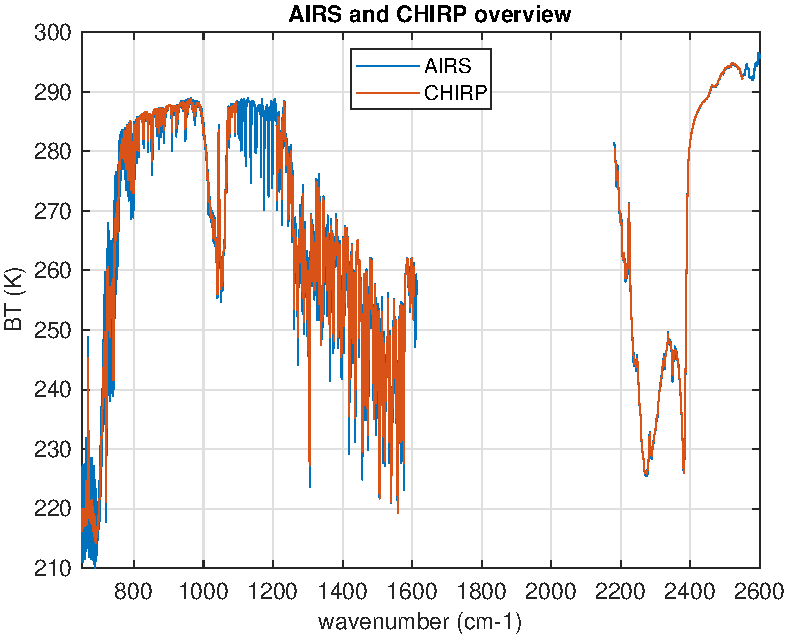
\includegraphics[width=\textwidth]{figures/airs_and_chirp_overview.pdf}
    \caption{Sample AIRS and AIRS-parent CHIRP spectra, granule means
      for 19 Aug 2018 granule 25.  The CHIRP bands are the intersection
      of the AIRS and CrIS bands.}
    \label{fig1}
  \end{minipage}\hfill
  \begin{minipage}[t]{0.45\textwidth}
    \centering
    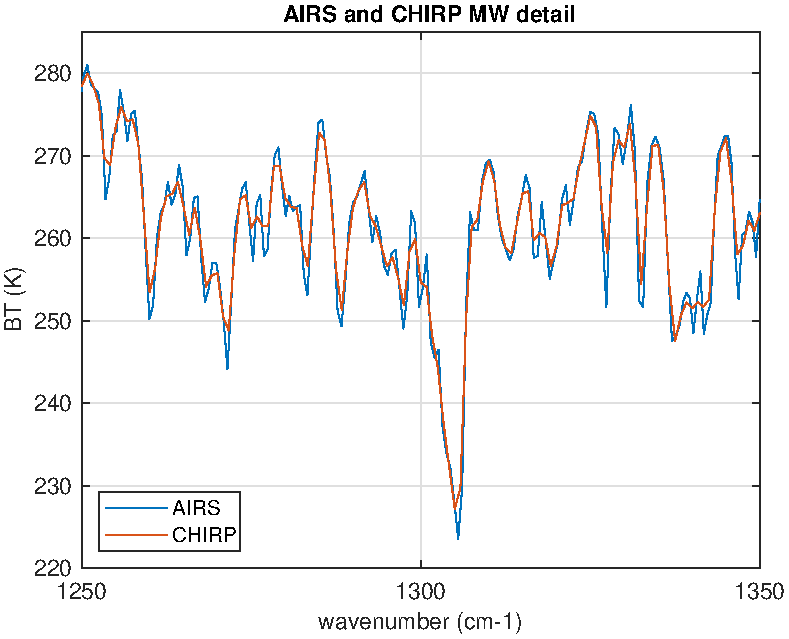
\includegraphics[width=\textwidth]{figures/airs_and_chirp_mw_detail.pdf}
    \caption{MW detail from the same granule.  Note that the data
      are on two different grids, and what we mainly see is the
      effect of the CHIRP apodization.}
    \label{fig2}
  \end{minipage}
\end{figure}

% CHIRP ILS
\begin{figure} % source a2cris_srfs.m
  \centering
  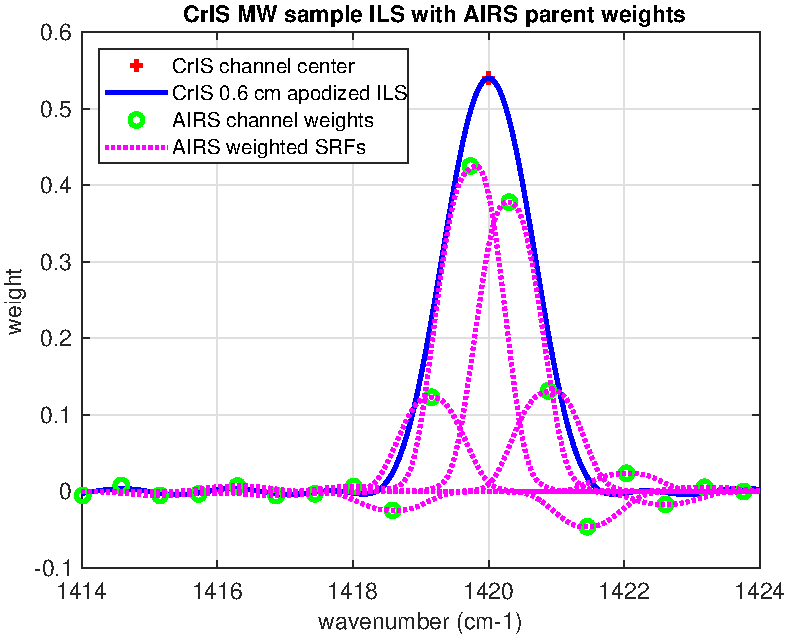
\includegraphics[height=9cm]{figures/sample_CrIS_ILS_with_AIRS_parent_SRFs.pdf}
  \caption{The MW CHIRP apodized ILS, together with weights for the
    AIRS channels, for the CHIRP channel shown.  The AIRS weights
    are paired with the corresponding AIRS SRFs, normalized to the
    weight values.}
  \label{fig3}
\end{figure}

For a long-term record we need radiance data in a single format---a
single frequency grid with a common ILS, and to the extent possible,
similar NEdN.  CHIRP radiances are for a nominal 3-band
interferometer with an {\opd} of $0.8$ {\cm} in the long-wave (LW),
$0.6$ {\cm} in the medium-wave (MW), and $0.4$ {\cm} in the
short-wave (SW) bands, with Hamming apodization applied to each band.
The MW and SW resolutions are lower than the CrIS-parent FSR {\opd}
of $0.8$ {\cm}, and were chosen to to give an approximate match to
the AIRS resolution for those bands.  Figure \ref{fig1} shows
typical AIRS and AIRS-parent CHIRP BT spectra, the granule means for
19 Aug 2018 granule 25.  The CHIRP bands are the intersection of the
AIRS and CrIS bands.  Figure \ref{fig2} is a MW detail from Figure
\ref{fig1}.  Note that the AIRS and CHIRP data are on two different
grids, and what we mainly see is the effect of the CHIRP
apodization.

For CrIS-parent CHIRP, we interpolate the CrIS Full Spectral
Resolution (FSR) product, with an $0.8$ {\cm} {\opd} for all three
bands, to the CHIRP grid and then apply Hamming apodization.  The
CrIS-parent CHIRP ILS is then a Hamming-apodized sinc for a $0.8$
{\cm} {\opd} in the LW, $0.6$ {\cm} in the MW, and $0.4$ {\cm} in
the SW.  Figure \ref{fig3} shows this ILS for a typical CHIRP MW
channel.

We want to match this ILS for the AIRS-parent data.  But AIRS is a
grating spectrometer with a distinct response function for each
channel, while CrIS is a Michaelson interferometer with a sinc
response function after calibration and corrections.  We use our
detailed knowledge of the AIRS spectral response functions to
deconvolve AIRS channel radiances to a resolution enhanced
intermediate representation.  This is done by taking a Moore-Penrose
pseudo-inverse of the tabulated AIRS SRFs and applying this to the
AIRS radiances, giving us deconvolved data at a $0.1$ {\wn} grid.
This is then reconvolved to the CHIRP user grid via resampling or
double Fourier interpolation.  The resulting translation can be
shown to be more accurate than more conventional interpolation or
regression \cite{mott2018}.  Figure \ref{fig3} includes the AIRS
chanel weights and corresponding AIRS SRFs, normalized to the weight
values, for AIRS-parent data for this channel.  The weights are from
a row of a linearized approximation of the AIRS to CHIRP translation.

Hamming apodization (as mentioned above) and an optional bias
correction are applied to both translations.  Currently AIRS and
CrIS J1 parent are adjusted to match CrIS SNPP \cite{strow2020a}.
After translation from CrIS, the three bands have 713, 649, and 317
channels, respectively.  These are concatenated for the CHIRP
product, for a total of 1679 channels, with frequency steps of $1/(2
\,\opd)$.  The \texttt{wnum} field is a 1679-vector which gives
channel frequencies, and \texttt{rad} is a 1679 by 12150 array of
radiance data.  (The dimension 12150 is the number of observations
in a granule, and is discussed in the next section.)  AIRS-parent
CHIRP uses the same channel set.  However the AIRS-to-CHIRP
translation gives only 1483 channels, due to slightly different band
spans.  These are embedded in the 1679 channel set, with missing
channels flagged, as described in section \ref{format}.

%----------- section --------------------------------------------------%
\section{CHIRP Sampling}
\label{sampling}

% one day track map
\begin{figure} % source plot_subpt.m
  \centering
  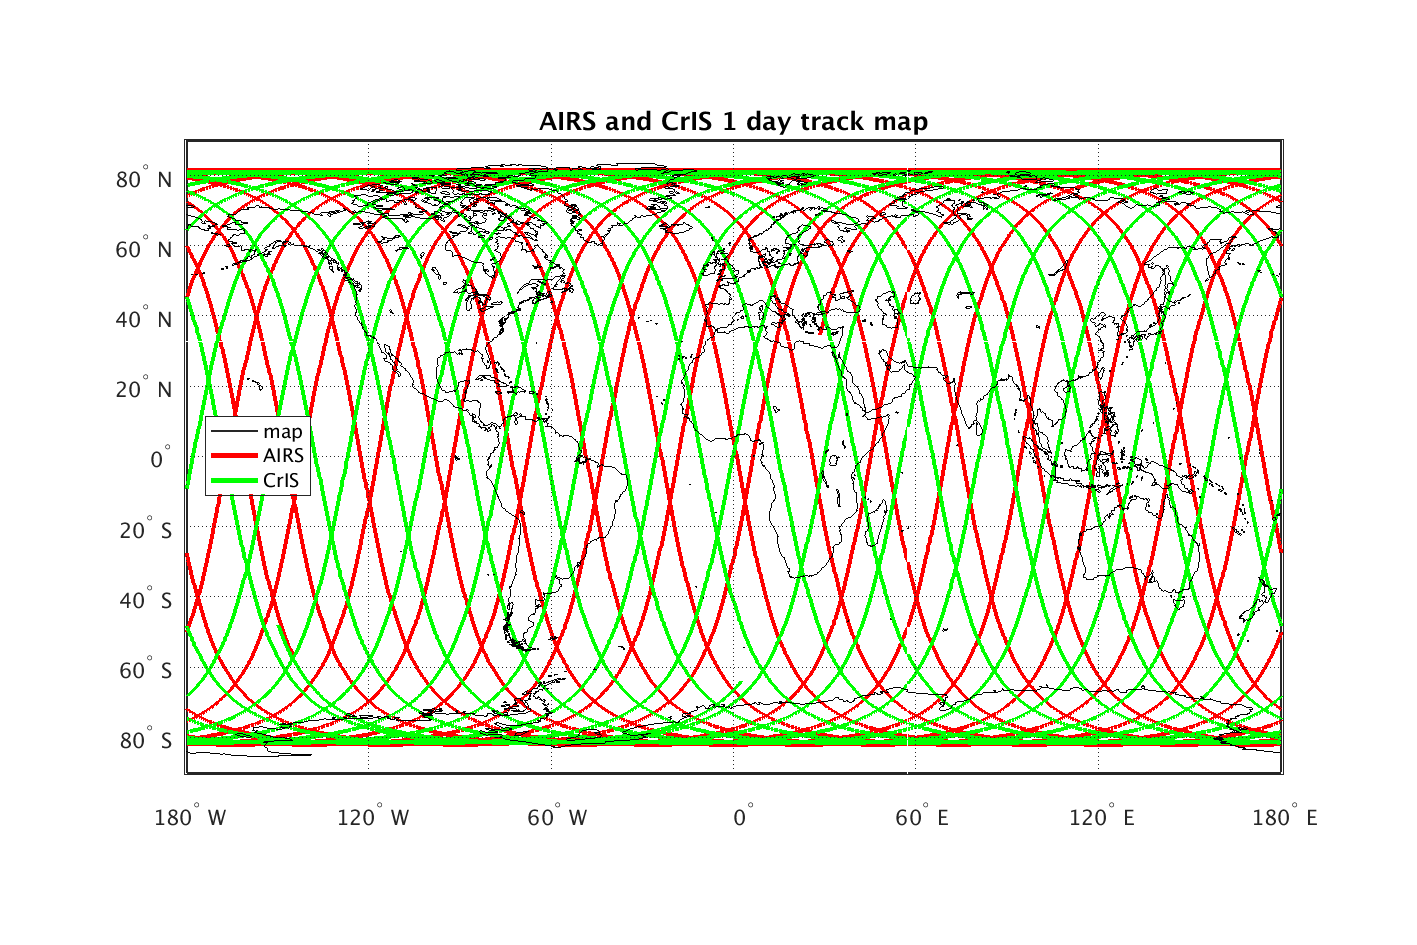
\includegraphics[height=10cm]{figures/subpt_1_day_all.png}
  \vskip-12mm
  \caption{Global one-day subpoint track map.}
  \label{fig4}
\end{figure}

% 16 day track maps
\begin{figure} % source plot_subpt.m
  \centering
  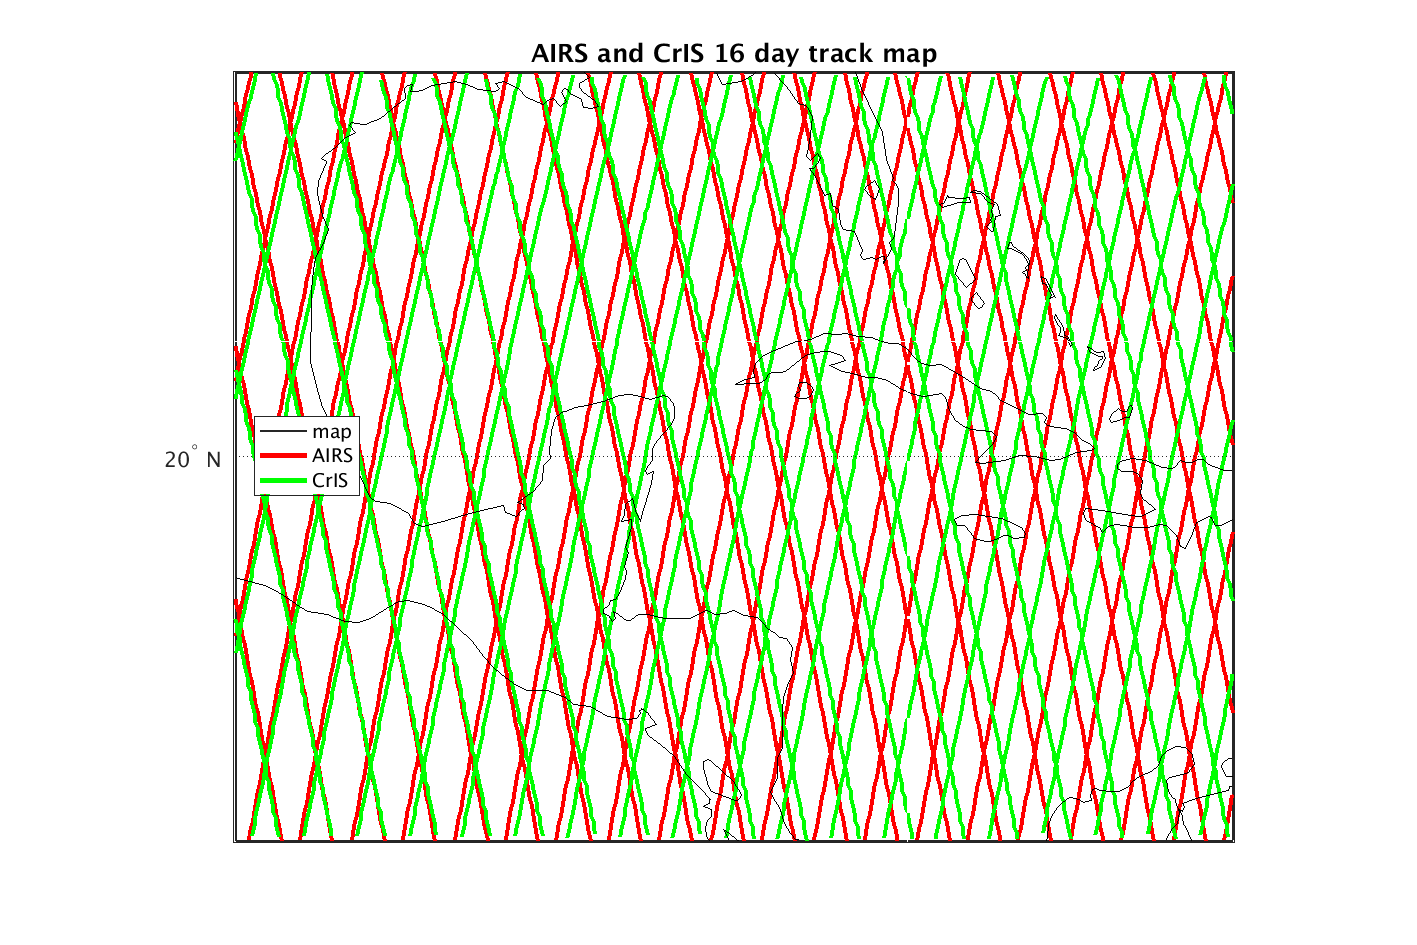
\includegraphics[height=10cm]{figures/subpt_16_day_zoom.png}
  \vskip-9mm
  \caption{Sixteen day subpoint track map for the Caribbean.}
  \label{fig5}
\end{figure}

% AIRS and CrIS secant of zenith angles
\begin{figure} % source plot_tbin.m
  \centering
  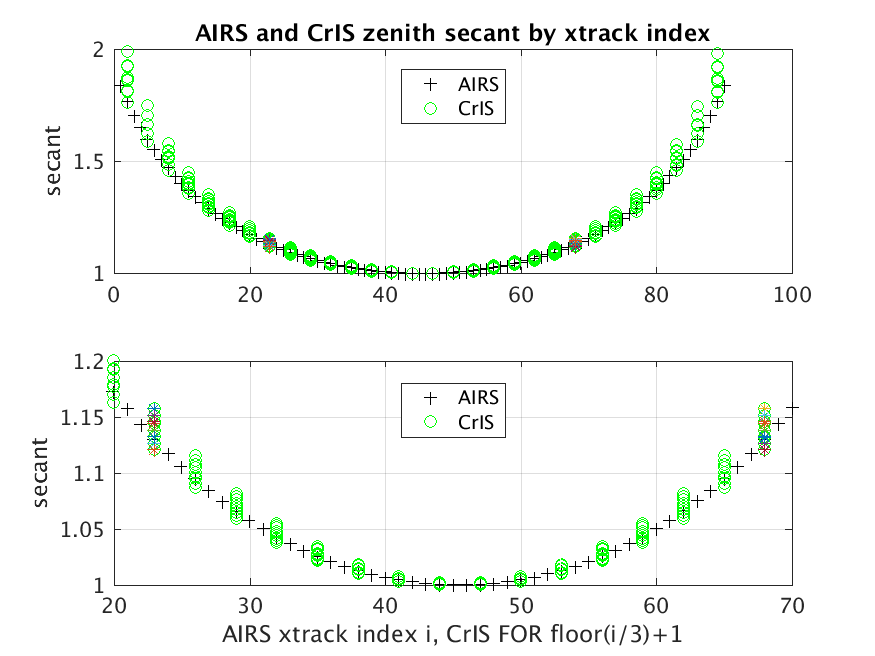
\includegraphics[height=10cm]{figures/AIRS_CrIS_secant_by_xtrack.png}
  \caption{AIRS and CrIS secant of zenith angles}
  \label{fig6}
\end{figure}

AIRS and CrIS are both in sun-synchronous polar orbits.  The CrIS
orbital period is 101.5 minutes $\pm 0.2$ seconds, giving 227 orbits
every 16 days.  The AIRS orbital period 98.8 minutes, giving 233
orbits every 16 days.  Note that 227 and 233 are both prime; there
are no common factors and so no repeating subpatterns.

Figure \ref{fig4} shows global values for satellite subpoint for
one day of AIRS and CrIS data, and figure \ref{fig5} for 16 days,
the full period before any repeated postitions, for the Caribbean.
AIRS and CrIS are cross-track scanners, and in addition to subpoint
tracks we need to compare the scan geometry.  Figure \ref{fig6}
shows the secant of zenith angles for AIRs and CrIS.  The upper plot
is for the full scan widths, while the lower is a near-nadir detail.
The general agreement is quite good, and the main difference we see
is due to the the CrIS FOV grouping.

Define an ``obs'' (observation) for AIRS as a single L1C 2645
channel radiance spectrum with an associated obs time, and for CrIS
as the the concatenation of the three radiance bands, giving $717 +
860 + 637 = 2214$ channels, again with a single associated obs time.
The AIRS L1c scan geometery is organized as 90 cross-track by 135
along-track observations, and so with 2645 radiance channels as an
$2645 \times 90 \times 135$ array.

The CrIS L1b scan geometery consists of 9 FOVs grouped in a $3
\times 3$ field of regard (FOR), giving 9 simultaneous observations,
with 30 cross-track FOR looks and 45 along-track steps.  With 2214
channels this can be represented as a $2214 \times 9 \times 30
\times 45$ array in the granule file.  (In practice this is broken
out by band, so we have a $717 \times 9 \times 30 \times 45$ array
for the LW, a $860 \times 9 \times 30 \times 45$ array for the MW,
and a $637 \times 9 \times 30 \times 45$ array for the SW.  But for
our basic counting here, we can simply use the concatenation.)
Note that $90 \times 135 = 9 \times 30 \times 45 = 12150$ obs per
granule, for both AIRS and CrIS.  AIRS and CrIS spatial sampling is
similar, but not identical.

%----------- section --------------------------------------------------%
\section{CHIRP Data Format}
\label{format}

AIRS L1c and CrIS L1b radiance data are organized as a sequence of
granule files, ordered by scan geometery and observation time.

Given our translations to a common 1679 channel radiance format,
the matching AIRS and CrIS obs count, with 12150 obs per granule,
and the generally similar sampling, we can define the CHIRP format
as an $1679 \times 12150$ array, channels by observation, in time
order.  Each ``obs'' has an associated values for time, FOV (for
CrIS), original indices for AIRS or CrIS, along with most of the
geo, support data, and product attributes from the parent sounders.
This involves some duplication of information for the individual
obs, but the overhead for this is small in comparison with the
radiance data.  CHIRP granules correspond with their parent AIRS or
CrIS granules, and inherit most of the parent granule's attributes
and supporting data.  CHIRP granules follow JPL conventions for
field names and attributes, and are saved in netCDF.

Aside from our basic CHIRP format, the representation as a list of
observations has some interesting applications.  For example we can
take a global tiling, and some time span, and associate each tile
with the obs that fall within it.  [CHIRP tiling is an obvious next
application.]

%----------- section --------------------------------------------------%
\section{Quality Control and NEdN Estimates}
\label{qcnedn}

CHIRP Quality Control (QC) is straighforward.  There are two QC
fields per granule, \texttt{rad\_qc}, a 12150-vector with one flag
value per obs, and \texttt{chan\_qc}, a 1679-vector with one flag
value per channel.  For both vectors, 0 = OK, 1 = warn, and 2 = bad.
For CrIS-parent CHIRP these fields are a summary of the parent
product state.  For AIRS-parent CHIRP the situation is more complex,
due to a significant and variable number of AIRS synthetic channels,
and because the set of 1483 channels from the AIRS translation is a
subset of the 1679 channels from the CrIS translation.

\subsection{AIRS-parent CHIRP QC}

For AIRS-parent CHIRP the 1679 element vector \texttt{chan\_qc} is
set to 2 (bad) for those channels that are not part of the 1483
channel set, as translated from AIRS.  This is a compromise that
lets us use a single freqency grid for CHIRP, regardless of the
parent sounder.  If we begin by choosing a set of channels to work
with AIRS-parent data, we can continue using that set with the
change to CrIS-parent, with no changes in our indexing.  In addition
to flagging missing channels, \texttt{chan\_qc} is set to 1 (warn)
for the six channels at the translation band edges, and when the
synthetic component exceeds a threshold, as described below.

The 12150 element vector \texttt{rad\_qc} has a flag for each obs.
These are set to 0 (OK) if the L1c field \texttt{instrument\_state}
is OK and radiance and geo values pass some basic sanity checks.
\texttt{rad\_qc} is always 0 or 2 for AIRS-parent CHIRP because AIRS
L1c doesn't have a warn flag.

\subsection{AIRS Synthetic Channels}

As an alternative to a warn flag, and to fill band gaps, AIRS L1c
provides synthetic values for some obs and channels.  These are
flagged in the L1c file for every obs and channel.  In addition,
for each L1c channel the granule file has a per-granule summary,
L1cNumSynth.  This is the number of times the channel was filled
with a synthetic value.  L1cNumSynth can range from zero, for no
synthetic values, to 12150, for all synthetic.  We are interested
in the synthetic fraction for channels from the CHIRP translation.
This is obtained as follows.  We linearize the AIRS to CrIS
translation and apply this to AIRS L1cNumSynth to get a
corresponding NumSynth values for CHIRP.  These are normalized as a
fraction and becomes the CHIRP field \texttt{synth\_frac}.  Then if
$\hbox{\texttt{synth\_frac}} > 0.25$, we set \texttt{chan\_qc} to
warn.  The threshold $0.25$ is a parameter that can be changed
in the production YAML specs.

Figure \ref{fig7} shows the sum of all synthetic obs by channel,
for 5036 consecutive AIRS granules, approximately 21 days of data.
Counts are shown on a log scale.  Figure \ref{fig8} shows the same
data as synthetic obs per channel, sorted by number of synthetic
obs. This shows the wide range of values, from few or no synthetic
obs for some channels, to entirely synthetic for others.  Figure
\ref{fig9} shows the AIRS-parent CHIRP synthetic fraction for a
single representative granule. This can be used to select channels
with a relatively small synthetic component.  Figure \ref{fig10}
show the AIRS-parent CHIRP synthetic fraction, sorted by synthetic
fraction magnitude.  This shows the variability of
\texttt{synth\_frac}.  As with L1cNumSynth, \texttt{synth\_frac} can
range from zero, for no synthetic component, to one, for entirely
synthetic.

\begin{figure}
  \centering
  \begin{minipage}[t]{0.45\textwidth}
    \centering
    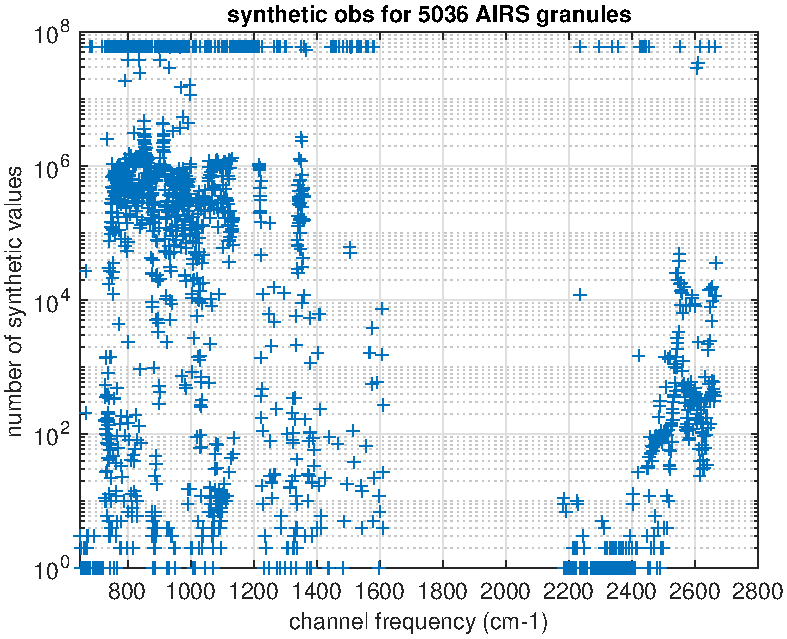
\includegraphics[width=\textwidth]{figures/synth_obs_freq_order.pdf}
    \caption{The sum of synthetic obs by channel for 5036 AIRS
      granules.  Counts are on a log scale.}
    \label{fig7}
  \end{minipage}\hfill
  \begin{minipage}[t]{0.45\textwidth}
    \centering
    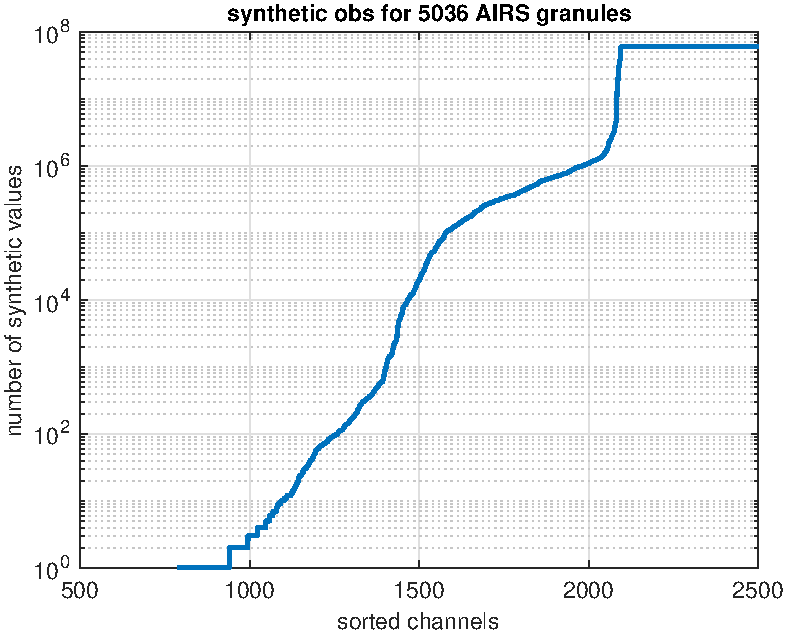
\includegraphics[width=\textwidth]{figures/synthetic_obs_counts.pdf}
    \caption{Synthetic obs per channel, sorted by number of
      synthetic obs.  This shows the range of values.}
    \label{fig8}
  \end{minipage}
\end{figure}

\begin{figure}
  \centering
  \begin{minipage}{0.45\textwidth}
    \centering
    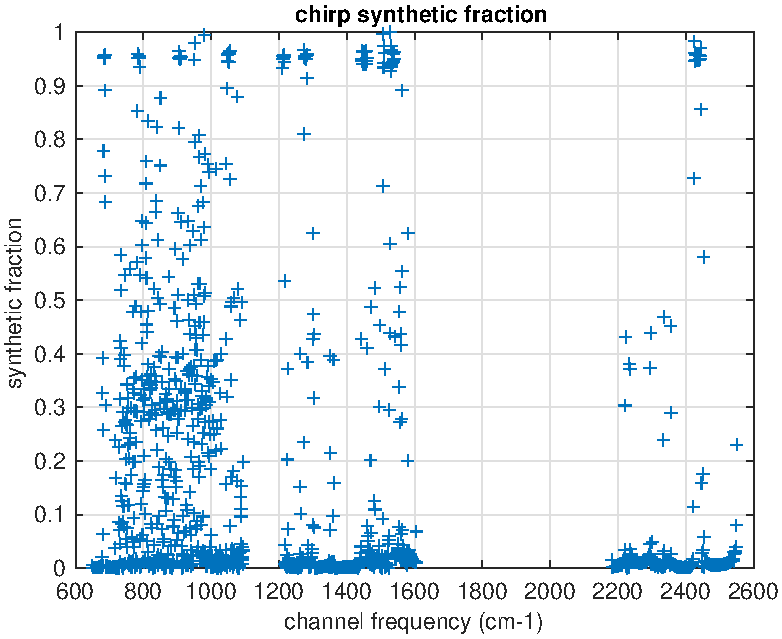
\includegraphics[width=\textwidth]{figures/chirp_sample_syn_frac.pdf}
    \caption{AIRS-parent CHIRP synthetic fraction for a single
      representative granule.  This can be used to select channels
      with a relatively small synthetic component.}
    \label{fig9}
  \end{minipage}\hfill
  \begin{minipage}{0.45\textwidth}
    \centering
    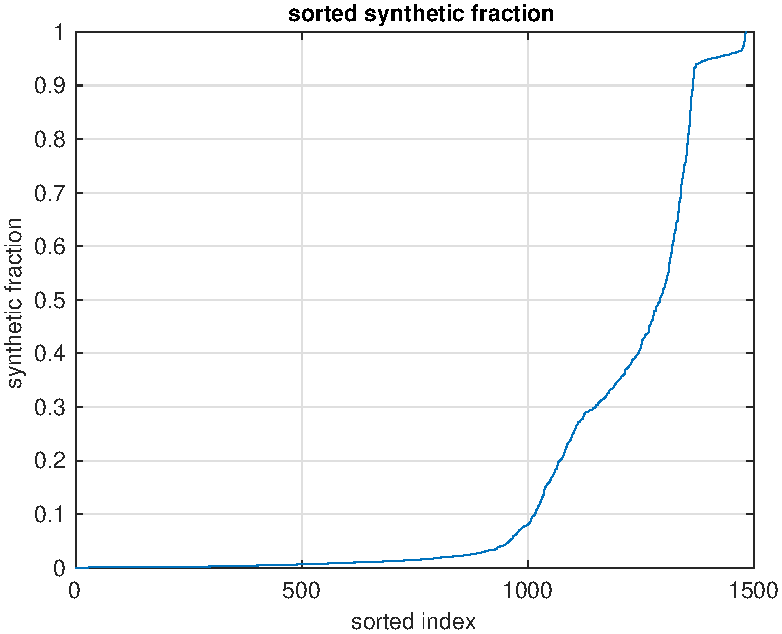
\includegraphics[width=\textwidth]{figures/chirp_sorted_syn_frac.pdf}
    \caption{AIRS-parent CHIRP synthetic fraction, sorted by
      synthetic fraction magnitude.  This shows the variability of
      synth\_frac.}
    \label{fig10}
  \end{minipage}
\end{figure}

\begin{figure}
  \centering
  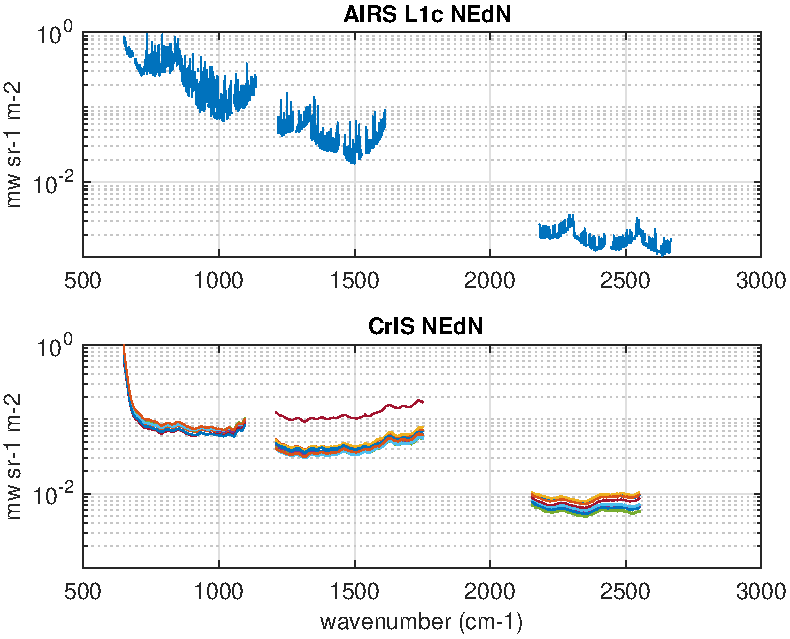
\includegraphics[height=10cm]{figures/sample_airs_and_cris_nedn.pdf}
  \caption{Sample AIRS and CrIS {\nedn} for the same two granules,
    2018 doy 231 granules 25 and 21.}
  \label{fig11}
\end{figure}

\begin{figure}
  \centering
  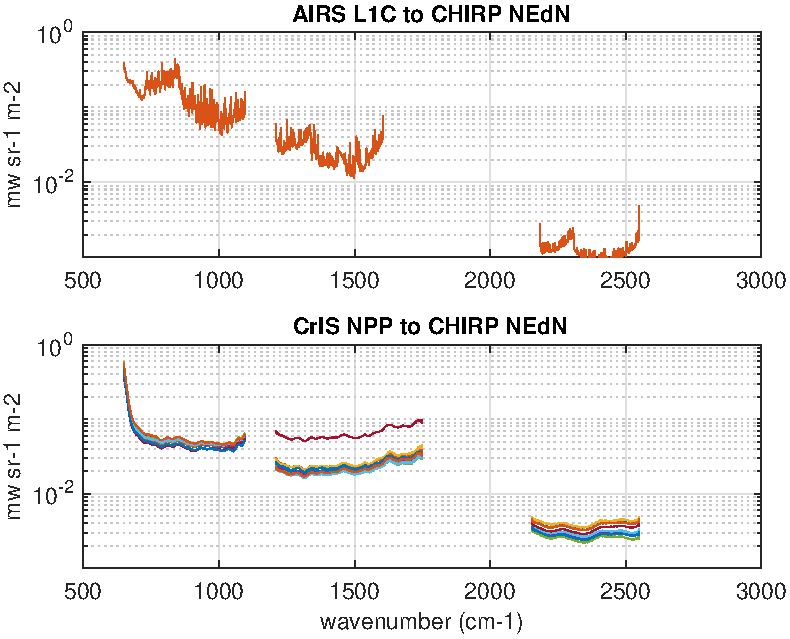
\includegraphics[height=10cm]{figures/chirp_nedn_from_airs_and_cris.pdf}
  \caption{Sample CHIRP {\nedn} for AIRS and CrIS parent data, 2018
    doy 231 granules 25 and 21, two relatively warm granules.}
  \label{fig12}
\end{figure}

\subsection{AIRS-parent CHIRP NEdN}

To find {\nedn} for AIRS-parent CHIRP, we start with an AIRS L1c
{\nedn} estimate.  Unfortunately the synthetic obs do not include
this.  To determine the effect of the translation on noise, it is
convenient to have at least a nominal value for {\nedn}, for every
AIRS channel.  So as a compromise we take the mean of valid {\nedn}
values over an AIRS granule, and interpolate over gaps from the
synthetic channels.

Given the AIRS estimate, we add noise at this spec to a black-body
spectra at 280K, do the translation, and measure the resulting
noise.  This is done repeatedly and the mean of the measurement is
reported.  Details are described in \cite{mott2018}.  Although a bit
involved, this only needs to be done once per granule, since we are
working from our per-granule AIRS estimate as described above.

The correlated fraction of AIRS noise varies from module to module,
and is significant for some modules.  The translation will preserve
this correlation.  {\nedn} estimates for such cases are a matter for
future work.

Figure \ref{fig11} shows typical values for AIRS and CrIS {\nedn}
for 2018 doy 231 granules 25 and 21, respectively; two relatively
warm granules.  Figure \ref{fig12} shows the corresponding CHIRP
{\nedn} for AIRS and CrIS parent data, for the same granules.
The noise is significantly less for the translation.  This to be
expected since both apodization and down-interpolation reduce noise.

[need to check and maybe expand on this a little.]

\subsection{CrIS-parent CHIRP QC and NEdN}

In comparison with AIRS, CrIS-parent CHIRP QC and {\nedn} is
relatively simple.  CrIS-parent CHIRP QC is determined from the CrIS
parent, by combining the fields for the individual CrIS bands.
\texttt{chan\_qc} is set to 0 (OK) for CrIS-parent CHIRP.  Possibly
we should set \texttt{chan\_qc} to warn at the band edges, as we do
for AIRS parent, but we are not doing this now.  CrIS-parent CHIRP
{\nedn} is derived from the high res CrIS {\nedn} with scale factors
to take into account the interpolation and apodization.  These are
\begin{itemize}
   \item LW, 0.6325, for Hamming apodization only
   \item MW, 0.5455, for interpolation and Hamming apodization
   \item SW, 0.4446, for interpolation and Hamming apodization
\end{itemize}

%----------- section --------------------------------------------------%
\bibliographystyle{abbrv}
\bibliography{user_guide}

\end{document}

